\documentclass[a4paper,16pt]{article}
\usepackage[margin=0.7in]{geometry}
\usepackage{sectsty}
\sectionfont{\huge\bfseries}
\subsectionfont{\LARGE\bfseries}
\usepackage{caption}
\captionsetup{font=large,labelfont=large}
\usepackage{graphicx}
\usepackage{listings}
\usepackage{subcaption}
\lstset{language=Matlab,basicstyle=\ttfamily\LARGE}
\begin{document}
	
	\pagenumbering{roman}
	
	\tableofcontents
	
	\newpage
	
	\section{Assignment 1}
	\vspace{0.2in}
	\subsection{Negative of an image}
	\indent	\lstinputlisting{negate.m}
	\begin{figure}[h!]
		\begin{subfigure}[h]{0.4\linewidth}
			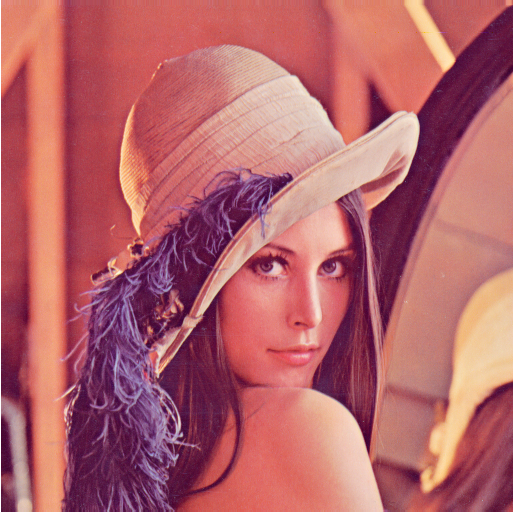
\includegraphics[width=\linewidth]{original}
			\caption{Original Image}
		\end{subfigure}
		\hfill
		\begin{subfigure}[h]{0.4\linewidth}
			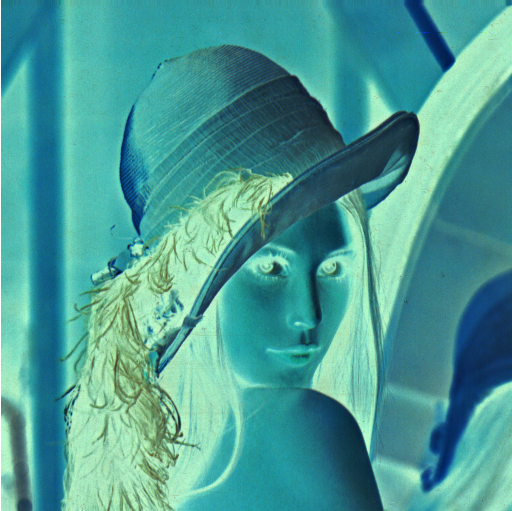
\includegraphics[width=\linewidth]{negative}
			\caption{Negative Image}
		\end{subfigure}%
		\caption{a normal and a negative image}
	\end{figure}
	\newpage
	\section{Assignment 2}
	\vspace{0.2in}
	\subsection{Plotting the histogram of an image}
	\vspace{0.2in}
		\lstinputlisting{his.m}
		\vspace{0.4in}
		\begin{figure}[h!]
			\begin{subfigure}[h]{0.4\linewidth}
				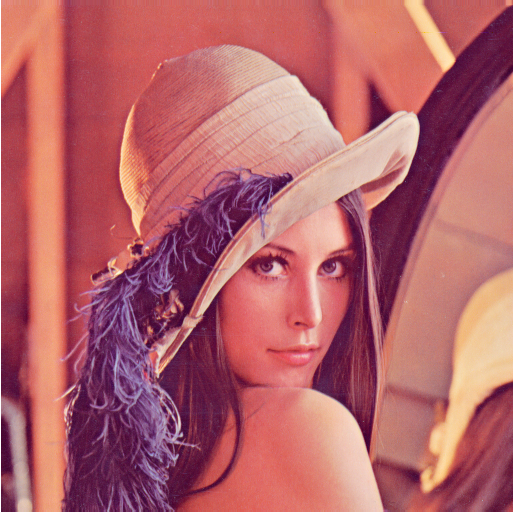
\includegraphics[width=\linewidth]{original}
				\caption{Original Image}
			\end{subfigure}
			\begin{subfigure}[h]{0.56\linewidth}
				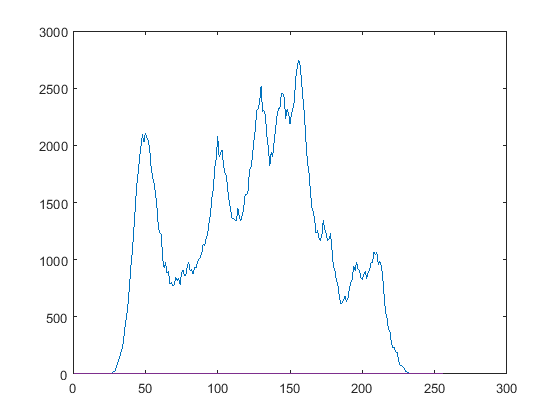
\includegraphics[width=\linewidth]{histogram}
				\caption{Histogram of the Image}
			\end{subfigure}%
			\caption{Image \& histogram of the image}
		\end{figure}
	\newpage
	\subsection{histogram equalization}
	
\end{document}
